\section{Strategy}
To recognize emotion first is needed to find a face in an image, at first I considered using LBP histograms but since I was interested only in facial expression's features seemed reasonable to use landmark points. 
Assuming that similiar expressions have a similiar position on different faces through an SVM classifier it could be possible to predict someone's "emotion" \footnote{As said earlier someone's emotions are more deep than just their facial expression.}.
For our purposes not all points where considered but only ones representing eyes and the mouth, this means only the points from 37 to 68 in figure \ref{fig:landmarks}.
In general to get good results is reccomended to use neural networks ~\cite{blog:emotion}, anyway I was interested SVM classifiers and how one would perform.

\begin{figure}[h!t]
    \centering
    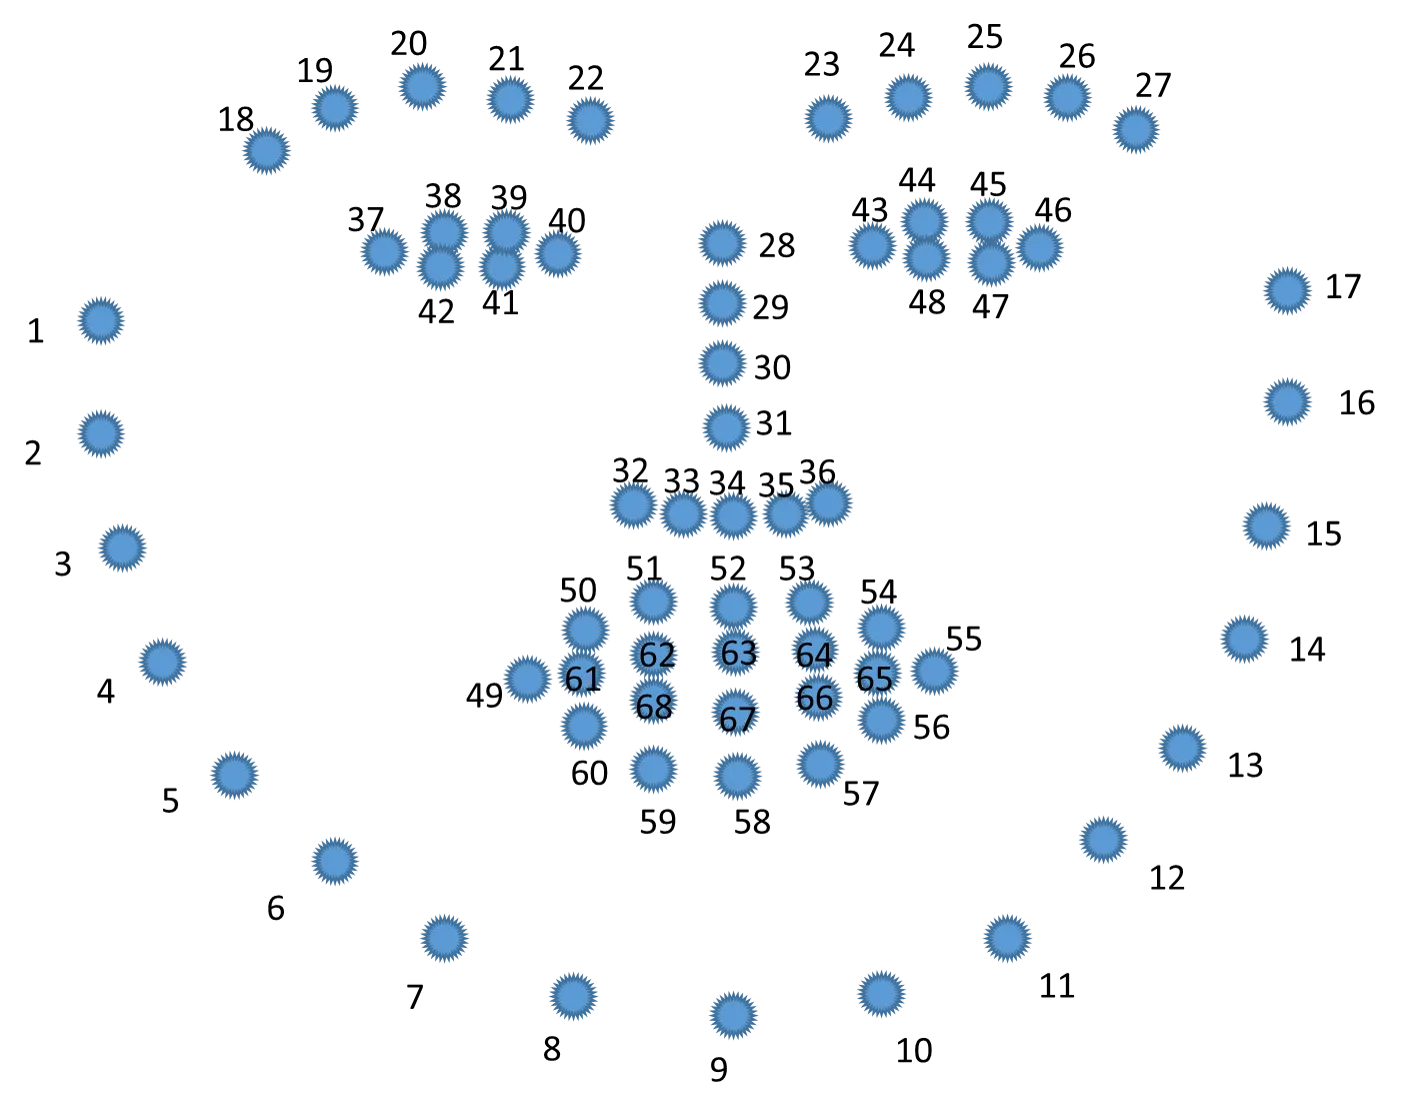
\includegraphics[scale=0.2]{images/landmark.png}
    \caption{Face landmark points from ~\cite{landmark:guide}.}
    \label{fig:landmarks}
\end{figure}

The adopted dataset is the \textit{First Affect-in-the-Wild} (affwild) ~\cite{dataset:affwild}, it consists of 298 videos of which 252 for training and 46 for testing.
Only videos in the train set have responses associated to them so I ignored the test set, for each video in which is identified a bounding box are associated the responses.
The emotion is definex as a point on a two dimensional cartesian plane where the $x$ axis is the \textit{valence}, it expresses if an emotion is positive or negative, and the $y$ axis is the \textit{arousal}, it discriminates animated emotions from languid ones as can be seen in figure \ref{fig:emotion_classification} where are defined only 4 different emotions but is possible to define more.
Considering I wanted to avoid classifying between too many classes -  with the risk of performances reduction - and considering also that SVMs in their purest form are binary classifiers, it came natural to me to just consider only response between valence or arousal and I chose valence.

\begin{figure}[h!t]
    \centering
    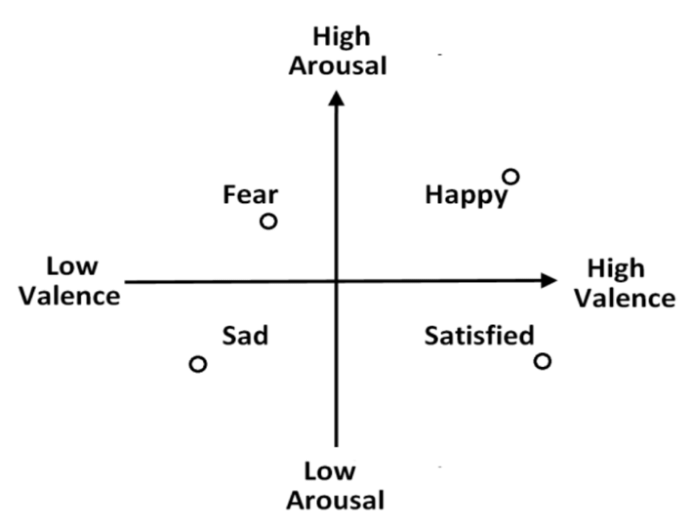
\includegraphics[scale=0.45]{images/emotion-classification.png}
    \caption{Emotion classification model from ~\cite{emotion_classification}.}
    \label{fig:emotion_classification}
\end{figure}
